\chapter{Related Work}
A spatial database system is a data management system for organizing and querying multidimensional spatial objects. Different from one-dimensional data, spatial data objects are often more complex and more informative. One dimensional data usually represents a point object on a single axis. In a multidimensional space, an object can be represented as line segments, polygons or a cluster of points arbitrarily dispersed in the space. It is problematic to represent such a spatial object in a fixed-sized data element. Since there is more than one dimension, the relationship between data values is also more complex. In a one dimensional dataset, we can easily sort the data in a particular order (ascending or descending), and repeated values are obvious to find. In a multidimensional space context, spatial objects can overlap, contain or union with each other, and the order of each object is not so obvious. 

Spatial objects are also dynamic \cite{Gaede:1998fp}. Insert, delete and update spatial values into the database system is required to be robust over time, and a spatial data index should embrace the changes dynamically. Operations in the spatial database system are much broader than traditional databases \cite{Gaede:1998fp}. The basic query operation can be retrieving points for given coordinates. The more complex ones are retrieving more than one point in the multidimensional space for a given range, or to check whether a point is contained within a spatial object. This can make a spatial index more difficult for handling different types of operations. 

The scale of the spatial database system can be large. Presenting multiple types of spatial objects at the same location might take more space because a spatial data index might use different data objects at this location. For example, a geographic map usually takes up a couple of gigabytes of memory. 

Properties commonly shared between one-dimensional data index and spatial data index are space and time efficiency. Data indexes are attempting to reduce the operations that are required for accessing the memory. For example, B-Tree \cite{Bayer:2002ds} is organizing data at a physical level to minimize the number of access to disk pages. The size of the data index should also be kept small to maximize storage utilization. 

Overall, designing an efficient, functional and dynamic spatial index requires considering all the tasks above. In the following sections, we will review the definitions of spatial queries and analyze some popular techniques in spatial data management systems, and spatial indexes that apply these techniques. 




\section{Spatial Queries}
We are assuming all the spatial queries are performing in two-dimensional spatial plane space. 

\begin{query}\label{def:pmq}
Point Match Query: given a point $p$ with a coordinate $(x, y)$ in the spatial extent ${p_{x, y}} \subseteq {E^d}$, find a exact point $p'$ within the same spatial extent as the $p$:
\[PMQ(p) = \{p|p'.x = p.x \land p'.y = p.y\}.\]
\end{query}

The most important and frequently used query in spatial data is the point match query. The Point Match Query searches for a spatial point for given coordinates, and it is a fundamental query for more complex queries.

\begin{query}\label{def:rq}
Range Query: given a two-dimensional area of interest $R = [p_{x_{min}}, p_{y_{min}}] \times [p_{x_{max}}, p_{y_{max}}]$, where $[p_{x_{min}}, p_{y_{min}}]$ is the coordinate of the lower-left corner of the bounding box, and $[p_{x_{max}}, p_{y_{max}}]$ is the coordinate of the upper-right corner of the bounding box. Find all points $p$ within or overlapping with the range $R$:
\[RQ(r) = \{p|(p_x, p_y) \cap R \neq \emptyset\}.\]
\end{query}

The Range Query retrieves multiple spatial objects that are within a window. The shape of a window is usually a rectangle, but it can be in other forms of shapes with arbitrarily unparalleled lines.

\begin{query}\label{def:nnq}
Nearest-Neighbor Query: given a point $p$ with spatial space $p\subseteq{E^d}$, find $k$ points $p'$ having a minimum distance from $p$:
\[NNQ(p) = \{p'|\forall p'':dist(p', p) \leq dist(p', p'')\}.\]
\end{query}

The Nearest-Neighbor Query is to find $k$ neighbour objects that are closest to the query point.  The distance functions for NNQ to compare the closest points include the Euclidean and Manhattan distance. 



\section{Spatial Indexing Techniques}
Many spatial indexes are developed based on one-dimensional methods. However, to fulfill requirements of query handling in spatial indexes, additional techniques such as transformation, overlapping regions, clipping and multiple layers are introduced in \cite{Faloutsos:1991ue}. 


\subsection{Transformation} \label{Transformation}
The transformation technique constitutes spatial objects (polygons, line segments, and so on) into a format of point, it can allow one-dimensional data management methods directly applied to spatial objects. The space-filling curves are examples of transformation, the continuous curve transforms two-dimensional data into one-dimensional while preserving the locality. Other methods including minimizing the spatial data object into points, x and y coordinates of two diagonal corners can be used for endpoint transformation; or a centroid point of the object with two additional parameters that measure width and length. However, the disadvantage of transformation is that firstly the range queries can be more complicated than in the original space. Secondly, the distribution of data can also have a larger chance to be non-uniform due to useless points. Thirdly, two objects that are close to each other in the original space can be arbitrarily apart in the one-dimensional space.  

\subsubsection{Space-filling Curves}
Space-filling curves can be used to represent a list of grid cells or, equivalently, a list of one-dimensional intervals that define the position of the grid cells concerned can be used to represent extended objects. It is especially useful for organizing multidimensional spatial data on one dimensional data access methods. How to order points on a grid layout and fill curves in between points is critical for an efficient data lookup. Popular space-filling techniques include the Z-ordering curve \cite{Orenstein:1984jq} and Hilbert curve \cite{Kamel:1994ux}. Both of them tend to arrange data as close to each other as possible, as well as in terms of memory space.

\begin{figure}[ht]
\centering
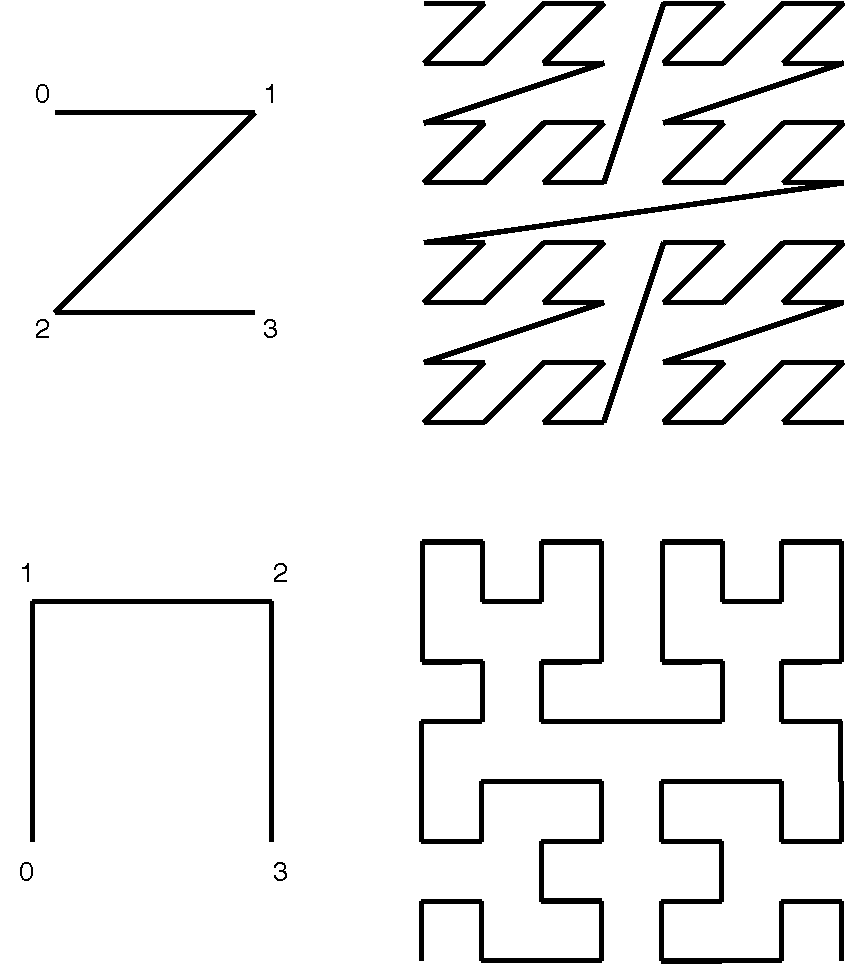
\includegraphics[scale=0.5]{Figures/space_curve.pdf}
\caption{Z-ordering Curve and Hilbert Curve}
\label{fig:space_curve}
\end{figure}

\paragraph{Z-ordering Curve}
Z-ordering \cite{Orenstein:1984jq} is a space filling curve dynamically hashing points that are close to each other, which is based on the Peano curve. The process of obtaining a z-ordering curve on a space starting from splitting into two equal sized subspace by ${(d-1)}$-dimensional hyperplane. This process can be executed recursively until it meets the following criterias \cite{Gaede:1998fp}. 

\begin{itemize}
    \item The current subspace does not overlap the data object.
    \item The current subspace is fully enclosed in the data object.
    \item Some given level of accuracy has been reached.
\end{itemize}

Each subspace can be represented by a unique z-ordering hashed bit string. To construct z-ordering bit strings in a coordinate system, one uses a bit interleaving the two binary values from the coordinates. For example, a value from a coordinate system can be represented as $(1, 2)$, the binary string for the two values is $001$ and $010$ respectively. The first value in the bit string comes from the first bit of the first value 1, followed by the first bit of the second value $0$. Therefore the first two bits are $01$, and the completed resulting bit string is $001001$. Z-ordered values created from the procedure are visually connected by a recursive z shaped curve. The resultant area collection is just an estimate of the initial entity. The accuracy and granularity (maximum number of bits) are required by the termination criterion. More Peano regions naturally will obtain more accuracy, but also sacrifice the size and complexity of estimating as a trade-off. The advantage of z-ordering is that spatial granularity shifts contribute directly to contextual improvements in the subsequent encoding. One drawback of z-hashing is that many useless data blocks will be created.

\paragraph{Hilbert Curve}
Another space-filling curve preserves locality well. Hilbert's order has been reported to be superior to the  Z-order curve as it has a better locality-preserving behavior \cite{Faloutsos:1991ue}. The Hilbert curve was first invented in 1891 by German mathematician David Hilbert \cite{hilbert1935stetige}. The fundamental idea is using a continuous line connecting the closest element in a grid, the difference between the Hilbert curve and the Z-order curve is that Hilbert is a U-shape curve. The transition from one column or row to the next is also choosing the closest cell rather than the diagonal cell in the Z-ordering curve. The U-shaped curve will be passed to the next cell in the grid in a similar manner, extending the continuous curve until the entire grid is filled in. The mapping of two-dimensional data stretches to the one-dimensional data layout, preserving the locality very well. It means that for points ${(x_n, y_n)}$ close to coordinates ${(x, y)}$, the output Hilbert value ${d_{x_n, y_n}}$ is also going to be closed to ${d_{x,y}}$. The Hilbert curve has been applied to the R-tree, combined with overlapping regions technique to improve the search performance. The Hilbert R-tree will be discussed in the latter part of the review. 



\subsection{Overlapping Regions}
Overlapping regions is a method that allows data buckets to access regions that have shared overlapped subspace. The linear transformation made point queries easier, but it is a challenge for handling range queries and containment queries without a complex spatial structure. However, redundant data can be created in overlapping regions, as a result, the number of search paths will be increased. Each insertion of new data can increase the overlapping area, eventually, overlap becomes too large for index searching efficiently. Therefore performance can be an issue for overlapping regions.

\subsection{Clipping}
Clipping has to be mutually disjoint, which does not allow overlapping between subspace. Consequently, the search path will only run through one path to the corresponding nodes instead of searching for multiple paths in overlapping regions. The major problem with clipping is also related to the insertion of new data. For new data that spans outside of the existing bucket region, a subdivision is required for subspace partitioning. This leads to a problem where more than one bucket has to be created for the same entry. The redundancy \cite{Orenstein:1989wy} can increase in the average search time, and also increase in the frequency of bucket overflow. Another problem with clipping is that when inserting new data, it can cause enlargement of the region if the region did not cover it. In certain circumstances, it is impossible to construct an enlargement without having an overlap between bucket regions. A new region has to be created due to overlapping is not allowed. This can potentially produce a much more complicated structure and problems with handling bucket insertion and overflow. Finally, due to splitting into smaller regions, the number of splitting regions will be increased. Hence, the database size is more likely to be large. 

\subsection{Multiple Layers}
Multiple layers \cite{Gaede:1998fp} are similar to overlapping regions, since regions in different layers can be overlapped. A hierarchical structure is usually used to combine with the multiple layers. However, data regions within a layer are disjoint, and it does not support extension to accommodate data objects. To insert a new data object, we attempt to find the lowest layer in the hierarchy structure that does not require to split. If such a layer exists, the data object will be inserted into that layer. If not, a new hyperplane will be introduced in order to split the new data region, then insert the data object to the new data region. Object will be moved to a higher layer, if it intersects the hyperplane. As we inserted more data into the structure, the higher layer will be collected on the higher layer, and the lower layers will have more segments of data objects. This can be inefficient for certain data distributions. Although, multiple layers still have advantage on selectivity of search path because of reduction of overlapping. 



\section{Traditional Spatial Data Indexes}

Characteristics of multidimensional data is complex  \cite{Gaede:1998fp, Robinson:1981id}. Gaede and Robinson have summarized some requirements for spatial indexes: dynamic, secondary storage management, a broad range of supported operations, independence of input data, simplicity, scalability, time efficiency, space efficiency, concurrency and recovery, minimum impact. The following sections introduce some of the popular traditional spatial indexing methods,  illustrate a wide range of techniques, as mentioned above, addressing the requirements for spatial index. 




\subsection{Grid File}

\begin{figure}[ht]
\centering
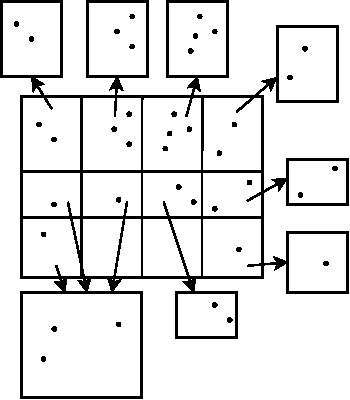
\includegraphics[scale=0.75]{Figures/grid_file.pdf}
\caption{Grid File}
\label{fig:grid_file}
\end{figure}

The grid file \cite{NievergeltJ:1984kc} is a hashing-based spatial access method, which is a grid layout partition to store data objects. A grid file consists of a rectangular d-dimensional cell, each grid cell has a number of shapes and sizes. A bucket contains one cell and many its neighbouring cells, and each cell is bound to one bucket. The main structure of the grid file consists of $d$ one-dimensional arrays called scales that are kept in the main memory. 


To perform an exact point match query, the first step is to access the location of the cell in the scale. Then the located cell will redirect to the reference of the page that contains all the potential points in that cell to perform an exact point match. The exact match query for the grid file is guaranteed to have 2 disk accesses. However for a range query, we must scan all cells that contain in the search region. 

Inserting a point to the grid file, the exact point match is also required. The matching query is trying to locate the cell, the point can be inserted if there is enough space. Otherwise we need to test if there is a hyperplane in the scale usable for separating data sections. When there is such a hyperplane a new data page must be generated and the data distributed accordingly. When no other hyperplane occurs, it would produce a splitting hyperplane. A new data page will then be generated, and the newly inserted point will be spread among the new data with the old data page. 


One of the major problems with grid files is dictionary split is expensive in high dimension, and even for uniformly distributed data it still has a super-linear growth of the directory. Some variations of the grid file tend to improve the structure and occupancy in the data buckets. EXCELL split the cell all in equal size, compared to the arbitrarily splitted space in the original grid file. The Two-Level Grid File added a level of grid file, limiting the splits without impacting too much of their surroundings to the subdirectory regions. The Twin Grid file introduced a second grid file parallel to the first one, which is a multilayer structure. The grid file has to create new data space by splitting thought hyperplanes when the number of points exceeds the limit. The twin grid file creates a new data space that requires redistribution of the data. 


\subsection{Multidimensional Linear Hashing}
MOLHPE proposed by Kriegel and Seeger \cite{Kriegel:vw} a multidimensional linear hashing with partial expansions to maintain order. This arrangement is based on the concept of extending the buckets in part without necessarily increasing the file size. Page address splitting depends on the page size from 0 to N, and a pointer p keeps track of the page. Two important contributions in building access methods. Firstly, whether a document remains in the old page or shifts to the new page only relies on the data key. Secondly, the old and the new sections will be filled in uniformly. Pages are united into groups to achieve a more evenly distributed loading factor. A group of pages will be expanded by one page once a new page has been added to the file. The file page expansion using an expansion pointer ${ep = (ep_1, \dots, ep_d)}$, and the address of the group is given by ${G(ep)}$. The expansion pointers will be updated along group partial expansion. 

It performed well over uniformly distributed data, outperformed many other spatial data retrieval systems. It overcomes the superlinearly growth of dictionaries in some multidimensional hashing methods such as the grid file. However, it does not handle very well on the non-uniform data distribution. A year later the same writers suggested linear order-preserving (PLOP) hashing to improve the performance on the non-uniform distributed data. The space partitions in PLOP are similar to the grid file, hyperplanes are organized by the binary tree. The d dimensional binary tree is also kept in the main memory just like the scale in the grid file. All the entries are stored in the leaf node, each leaf node from the binary tree is linked to each other for speedup.  




\subsection{K-D-Tree}

\begin{figure}[ht]
\centering
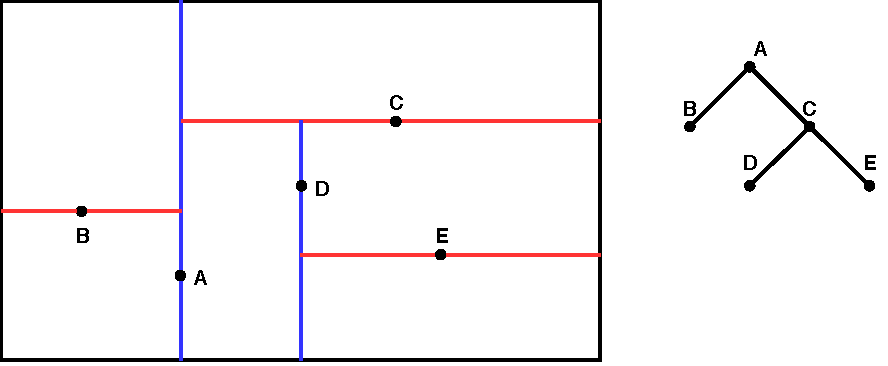
\includegraphics[scale=0.75]{Figures/kdtree.pdf}
\caption{K-D-Tree}
\label{fig:kdtree}
\end{figure}

K-D-Tree \cite{Bentley:1975gn} is a popular multidimensional data scheme that uses a hierarchical structure. It is a binary search tree, and each node represents a point in ${K}$ dimensional space. The universe of ${K}$ dimensional space is splitting by ${K-1}$ dimensional hyperplanes recursively. Each data point is used as the coordinate of splitting hyperplanes, which depends on whether the node is X-align or Y-align. The X-align or Y-align decides which axis to compare for newly inserted data points. The intermediate nodes have one or two descendants for search. The searching procedure is straightforward, comparing the corresponding axis value from the tree level, then going to the right or left subtree, repeating the process until the goal data point is found. 

One of the problems with the K-D-Tree is that the order of inserting points can have a large effect on the shape of the tree. Also, data points are distributed scattered over the tree, which will be difficult to execute complex queries such as the nearest neighbours query. Keeping the tree balanced can also be hard since the structure of the tree is mostly decided by the order of insertion. 

The adaptive K-D-Tree \cite{Bentley:1975gn} improves on the splitting by choosing the point that between points are evenly distributed on both sides. The splitting point is no longer taken from data points, data points are only stored in the leaves. Intermediate nodes store the coordinates of splitting points and the dimension information. It improves the original structure trying to store point values evenly, but it is still sensitive to the order of points being inserted. 


\subsection{BSP-Tree}

\begin{figure}[ht]
\centering
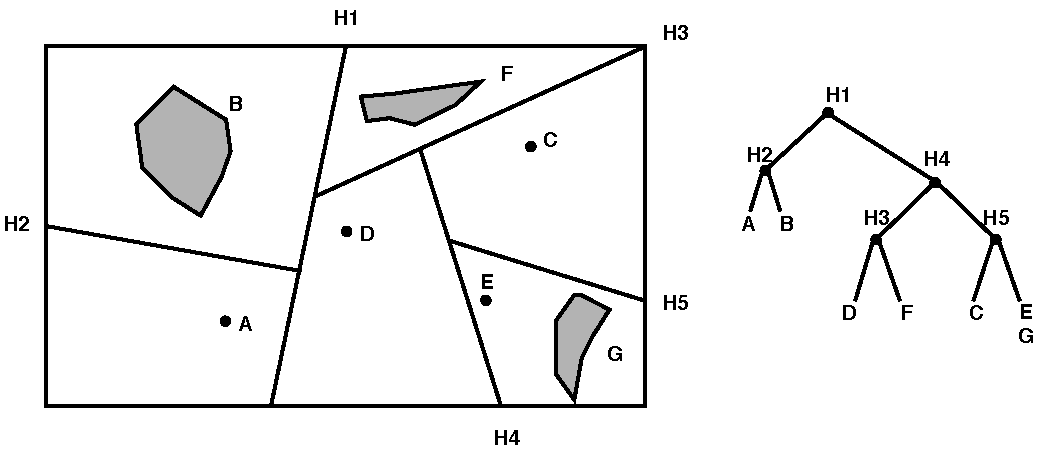
\includegraphics[scale=0.75]{Figures/bsptree.pdf}
\caption{BSP-Tree}
\label{fig:bsptree}
\end{figure}

Comparable to K-D-Tree, the BSP-tree \cite{Fuchs:1980bj} is also a binary tree with a recursive subdivision subspace by splitting hyperplanes. Instead of vertical or horizontal lines in the K-D-Tree, the BSP-tree uses the arbitrary orientation of splitting hyperplanes. It allows the subdivided space to be more flexible and well suited for arbitrary shapes of spatial objects. Since data points are not used as the splitting hyperplane, each subspace can be divided independently. The partition hyperplane can be selected depending on the distribution of data objects. 
Inserting a point to the tree is also similar to the K-D-Tree. Starting from the root node, the search point has to compare with the value in the root node and determine whether to go to the right or left part of the tree. All data objects are stored in the leaf node, so the search will stop until reaching the leaf node of the tree. 
The BSP-Tree can handle non-uniformed distributed data well. However, arbitrary splitting hyperplanes also require more complex calculations and storage space. 



\subsection{Quadtree}

\begin{figure}[ht]
\centering
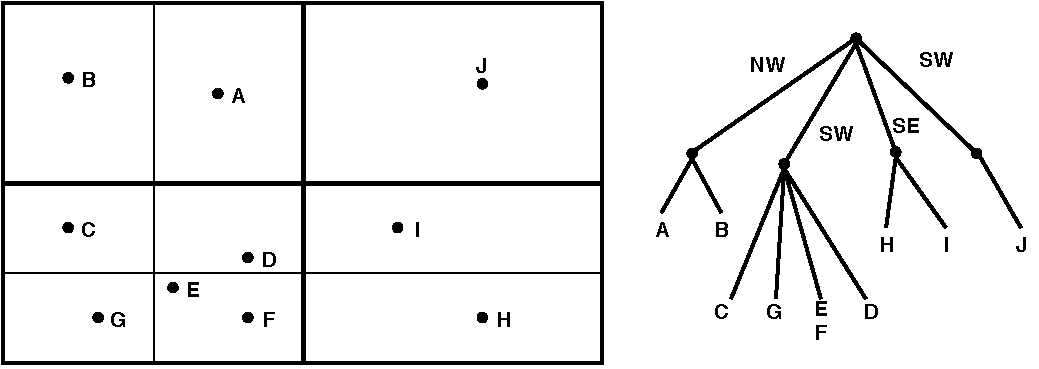
\includegraphics[scale=0.75]{Figures/quadtree.pdf}
\caption{Quadtree}
\label{fig:quadtree}
\end{figure}

The Quadtree \cite{CSUR:tm} is also considered to be closed to the K-D-Tree. The difference is the Quadtree is not a binary tree anymore. The intermediate node in the Quadtree will have ${2^d}$ descendants for d dimension. For example, d=2 will have four descendants, which each of the descendants is referred to as a rectangle region. These four descendants can be viewed as quadrants that represent four directions(NW, NE, SW, SE) prospectively. The recursive subdivision will be continued on the rest of the data. Consequently, the Quadtree will not be balanced since that more densely the region is deeper the tree will grow. 

Searching and inserting in the Quadtree is similar to other tree structures. New data points will start from the root node, the node will decide one subtree from the four descendants. For point query, there always will be only one candidate subtree for further searching. For range queries, there might be one or more candidate subtrees. The process will continue recursively until finding the goal.


\subsection{R-Tree}

\begin{figure}[ht]
\centering
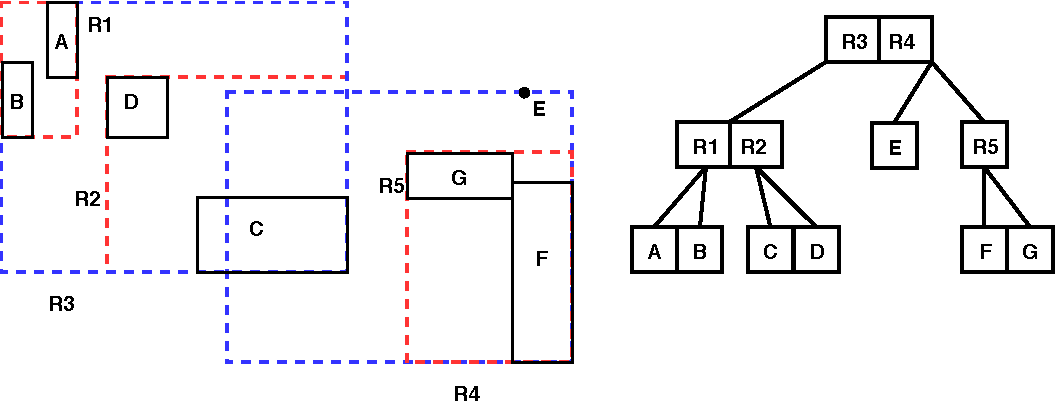
\includegraphics[scale=0.75]{Figures/rtree.pdf}
\caption{R-Tree}
\label{fig:rtree}
\end{figure}

R-Tree\cite{Guttman:1984ka} is a height-balanced hierarchical data structure that applies overlapping technique. Only the leaf nodes store the minimum bounding box (MBB) of data objects. For the interior nodes, each node has to store two information: children of the node and a MBB that contains all the nodes. The R-Tree contains the following properties: 

\begin{itemize}
  \item Each leaf node contains between m and M index records, except the root node. 
  \item For each entity in a leaf node, a minimum bounding box is used to contain the n-dimensional data object.
  \item The root node has at least two entries unless it is a leaf.
  \item All leaves are at the same level.
\end{itemize}


The increase of branching factor ${m}$ will decrease the tree height and improve space utilization because most of the space will be used in the leaf nodes. Searching in R-Tree is similar to the B-Tree. At each node in the tree, they will be tested if within the search ranges. Since the bounding boxes in R-Tree can be overlapped, the search path can go through more than one subtree. Because R-Tree only stores MBBs, the search result is not an exact match result. For actual spatial context data, we need to search further within MBBs.

Insertion in R-Tree is also similar to B-Tree. The newly inserted object first recursively finds a path to the leaf node starting from the root node. If the leaf node is not full, insert the new object. Otherwise, the leaf node has to be split by a splitting heuristic. The old objects from the original node will be distributed among the original and new nodes. We can adjust the tree by propagating the newly added nodes up and change the height of the tree. 

For the deletion of a node in the tree, the search query must be performed. If found in a leaf node, then delete it from the node. If there is not an underflow, the MBB will resize according to the updated nodes. If it causes an underflow, and the node occupation below ${m}$, then adjusting the tree is needed, the subtrees of the node will be dissolved and these nodes will propagate upwards. Old entries in the node will be inserted into a new temporary node or another option is to merge with siblings node. In both options, the tree has to adjust the MBB size and propagate upwards. 

To reduce the overlaps in insertion, the author proposes several different splitting algorithms in the original paper. A quadratic-cost algorithm picks two of the M+1 entries as the first elements of the two new groups. The criterion of choosing the pair is that they would take most areas if both were put in the same group, which means the region of a rectangle covering the two entries, minus the region of entries themselves, would be the largest. A linear-cost algorithm is similar to the quadratic-cost algorithm but uses different criteria to select the two entries. The two entries were selected based on the dimension of entries. For entries whose highest low side and lowest high side, record such separation. The separation will be normalized by the width of the entire set along the corresponding dimension. Then choose the pair with the greatest normalized separation along any dimension. 

\section{Learned Indexes for One-dimensional data}
\subsection{The Recursive Model Index}

\begin{figure}[ht]
\centering
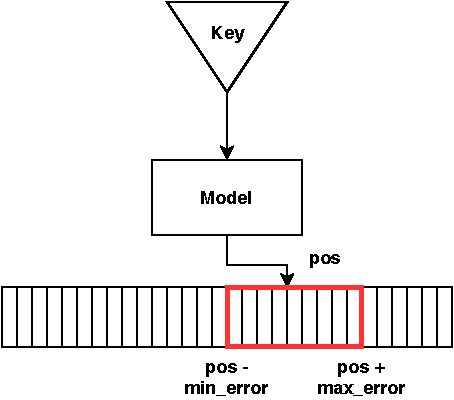
\includegraphics[scale=1]{Figures/rmi.pdf}
\caption{RMI}
\label{fig:rmi}
\end{figure}

 Kraska \cite{Kraska:2017vh}  proposed a method that uses a machine learning model to replace indexes. Kraska introduced the idea that data indexes can be treated as models, we can describe the data distribution by constructing the cumulative continuous functions. A B-Tree indexes a key into a hierarchical structure, retrieving the position of that key from traversing the tree. It stores as many as children as possible to diminish the height of the tree, hence to reduce the number of disk access. The B-Tree is a self-balance tree, it only provides an approximate position with min and max error with stored keys. The optimal searching time complexity requires log time retrieval. To insert and delete a key, B-Tree needs to re-balance to provide the same search time guarantee. More importantly, strong error bounds are not needed since prediction results can be replaced by local precise search algorithms. Identical patterns obtained in a continuous function that used to describe a distribution of data can be used to build a data structure for indexing. As a result, range searching in the B-Tree index can be replaced by machine learning models such as linear regression, which can predict an approximate point to the next stage and error from the prediction does not affect the final search accuracy. 

\[p = F(Key) * N\]

The CDF models data distribution and predicts the position of the key as shown above. P is the predicted position, F is the cumulative distribution function estimate likelihood for a range observed key and N is the total number of the key. The learned index is optimized by learning the CDF and minimizing the error from the linear regression model. The recursive-model indexes (RMI) is a series of machine learning models on a hierarchy structure. The RMI consists of multi-stages, where the model predicts a value from the input key at each stage. Due to range indexes that can point to a range of values, the predicted value does not need to be exact. The predicted value can be the final position result if at the final stage of the structure or a pointer to the next stage if it is not the final stage. 

In the experiment, the recursive model can be built by a mixture of machine-learned index models and B-Tree. For a 2 stage model: the top stage is a 2 layer fully-connected neural network with 32 neurons per layer with the ReLU activation function, and the second stage can be thousands of simple linear regression models or B-Tree. The data distribution learned by the model can give a prediction of the pointer, the pointer is pointing to a specific range of values in the next stage. All models at final stages are trained by a specific range of values, and have much better accuracy for values within that specific range. In other words, we are reducing the searching range of values at each stage. However, like most neural net models, the prediction value can have uncertainty with min-/max-error. In the case of the neural net model performing worse than a threshold, the neural net model can be replaced by a B-Tree to ensure the ‘last-mile’ accuracy. 

Two search strategies mentioned in the paper, one is the model biased search and another is biased quaternary search. The model biased search is a simple binary search that it set the middle point of as the predicted value from the model. Tha biased quaternary search takes ${pos - \sigma}$, ${pos}$, ${pos + \sigma}$ as the initial three points, which can make the initial guess as accurate as possible. The min- and max-error sets upper and lower bounds that can guarantee all the points can be found. However, a wrong lower or upper bound can be generated for non-monotonic RMI models if the key does not exist. 

Kraska also discussed some applications of the learned model on other data structures.  The learned hashmap is trying to use a CDF to replace the hash function. The result shows the learned hashmap can reduce the number of conflicts by up to 77\% on a certain dataset. Kraska suggests that for a uniform distributed dataset, the linear model is no better than a randomized hash function. For small keys, traditional hash functions with Cuckoo hashing provide the larger payload and reduce conflicts from distributed hashmaps. 



\subsection{ALEX}

\begin{figure}[ht]
\centering
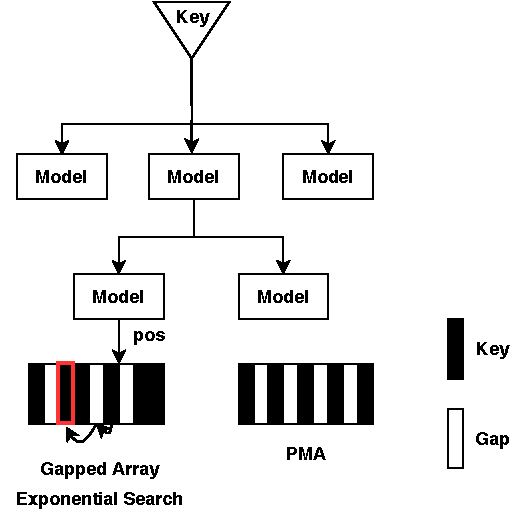
\includegraphics[scale=1]{Figures/alex.pdf}
\caption{ALEX}
\label{fig:alex}
\end{figure}

The ALEX \cite{Ding:2020wo} is an adaptive learned index improvement of the RMI. The major improvement is that ALEX uses different data structures to store data on the leaf nodes, whereas RMI uses only one single array. Gapped Array (GA) and Packed Memory Array (PMA) are the two node layouts that have been explored in the paper. Since all the data are stored in the leaf node, the search method in ALEX uses exponential search. The other feature is that ALEX adjusts the shape and height of the RMI dynamically depending on the updated workload. It also inserts records dynamically, which stores the key at where the model predicts. 


Gapped Array is one of the node layouts that use the idea of exchanging extra storage for the speed. It creates a gap during insertion to maintain good exponential search, then utilize the gaps with adjacent keys. To insert a new key into a gapped array, we must find the insertion position. RMI is used to predict the insertion position, if this insertion position is maintaining the sorted order, and is a gap, then the new key is placed to the gap and finish. If the predicted insertion position is not right, we have to use an exponential search to find the correct insertion position. The correct insertion position must be a gap to insert the new key. If it is not a gap, we shift the elements at this position by one position in the direction of the closest gap. The insertion performance achieves ${O(logn)}$. One procedure during insertion is if a new key pushes into the gapped array and exceeds the density bound ${d}$, then the gapped array needs to expand. A disadvantage of gapped arrays is when inserting a long contiguous region without any gaps, such \emph{fully-packed region} can cause a dramatic increase in the insertion time. 

Packed Memory Array is another node layout that has been shown to adopt and grow better to insert. The PMA is an array whose size is always a power of 2, and it divides itself into powers of 2 numbers of segments. The PWA builds an implicit binary tree, each segment is a leaf node and the root node represents the entire array.  Each node will have a density bound that can determine the maximum number of elements to the position in the region of the array. The size of PWA will expand once the density in the array becomes too full. The rebalance local portions of the PWA allows data to be uniformly distributed. 

Adaptive RMI Initialization in ALEX sets a predetermined maximum bound for the number of keys in a leaf node so that ALEX can determine the RMI depth and the number of leaf models adaptively. The root node will be divided into a certain number of partitions, and each partition will have exactly the maximum number of keys. Node splitting on inserts is another optimization in ALEX. If the new key will push to the leaf node exceeds the maximum bound, then we can split the node. The corresponding leaf node will become the interior model, and a number of children nodes will be created from the model. This allows the ALEX to start with empty data, and the RMI will grow deeper along with more inserted nodes.


\subsection{The PGM-index}

\begin{figure}[ht]
\centering
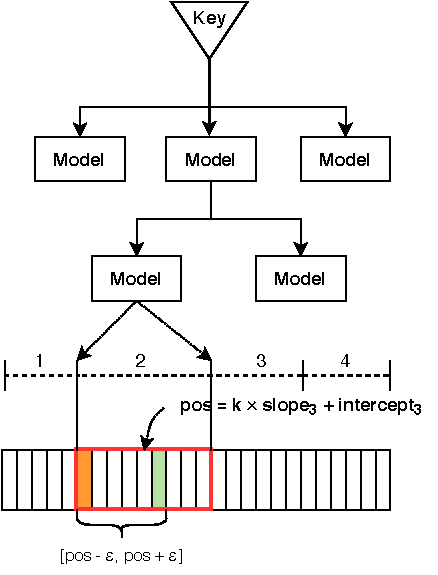
\includegraphics[scale=1]{Figures/pgm.pdf}
\caption{PGM-index}
\label{fig:pgm}
\end{figure}

The Piecewise Linear Approximation model \cite{Ferragina:ud} is a pure learned data structure, rather than a hybrid learned model such as RMI. The PGM-index builds upon a sequence of segments, each one indexing a sequence of keys in constant space and constant query time to return the approximate position of the key in the array. Another property of the PGM-index is it is a recursive algorithm that constructs the index structure to fit the distribution of the keys. 

The PGM-index is to focus on optimizing space-time trade-off. It has the following advantages in space-time complexity:

\begin{enumerate}
    \item Since the PGM-index is built upon the minimum number of segments from bottom-up, which is more efficient than other learned indexes in terms of time and space. 
    \item The PGM-index uses these segments as a constant-space routing table, rather than storing large number keys depending on the disk-page size in other learned indexes. 
    \item The routing tables in the PGM-index take constant time to limit the search of a key in a node to a smaller subset of the indexed keys.
\end{enumerate}

 The author provides compression algorithms to reduce the number of distinct slopes to their optimal minimum number for the compressed PGM-index. The multicriteria PGM index exploits the space-time flexibility by optimizing in two different criteria: 
\begin{enumerate*}
  \item Given a space constraint the output PGM that minimizes the query time.
  \item Given a maximum query time the output PGM that minimizes the space.
\end{enumerate*}
The number of $\varepsilon$-approximate segments controls trade-off between the space and time. The space occupancy decreases with increase of $\varepsilon$, whereas the query time ${t(\varepsilon)}$ increases with increase of $\varepsilon$. 

The performance result shows that the PGM-index improves space occupancy by offering theoretical bounds, and it guarantees a 4X increase in the precision of the estimated position of the searched key compared to the RMI. The PGM-index is reported to provide better latency guarantees since it can dynamically adapt to the data distribution, and it can use the ${\varepsilon}$-approximation to optimize a better performance trade-off between space and time.


\subsection{RadixSpline}

\begin{figure}[ht]
\centering
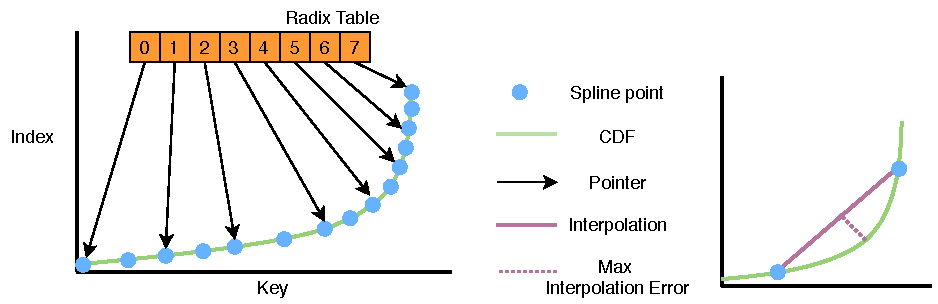
\includegraphics[width=\textwidth]{Figures/radixspline.pdf}
\caption{RadixSpline}
\label{fig:radixspline}
\end{figure}

RadixSpline \cite{Kipf:2020wr} is another learned index that builds upon a single pass over the data. RadixSpline is built in a bottom-up approach in two steps. First, a linear spline is to model the cumulative distribution functionc (CDF) of the data, which guarantees certain error bounds. Second, a radix table will be built as an approximation index into the spline points. 

To build a RadixSpline, we first construct an error-bounded spline model $S$ on top of the underlying data. The spline model $S$ always predicts the correct location of the data within a constant error of $e$. The parameters of the model $S$ are a set of spline data points $Knots(S)$. For any look up key $k$, linearly interpolating between the two closest spline points in $Knots(S)$ will output an estimate within error $e$. 

Then, the selected spline points are built to index in a radix table. The radix table can quickly find the two spline points surrounding the lookup key. It is a flat $uint32_t$ array that maps fixed-length key prefixes (“radix bits”) corresponding to the first spline point. The radix table uses $r$ as a parameter, so array size will be ${2^r}$. To increase the precision, the size of the array ${2^r}$ will grow exponentially with growth of $r$. The RadixSpline supports single pass building CDF, that means the sorted data points are passed in the spline construction and radix table allocation at the same iteration. 

Lookup in the radix table takes following procedures: first to extract an $r$-bit radix prefix $b$ from the key. Then, we can use the $b$ radix prefix access to the radix table retrieving two spline points. A linear interpolation will be performed between two spline points to find an estimated position $p$ of key. Finally, it uses a binary search to find the first occurrence of the key within the error bound $(p \pm e)$

The building performance of RadixSpline is significantly lower than the RMI. In lookup latency, RadixSpline performs similarly with RMI, which both are better than traditional indexes such as B-Tree. However, the lookup latency of learned indexes can be affected by the distribution of the dataset. The index size of RadixSpline is unstable for different dataset, the paper reports significantly high memory cost in one of the dataset. 

\subsection{FITing-Tree}
FITing-Tree \cite{galakatos2019fiting} is another learned index that uses a piecewise linear function for key index approximation. The idea of the FITing-Tree is to partition keys into fixed-sized segments within certain error bounds. The error is defined as associated with the maximum prediction error distance between the actual position and the predicted position. Two types of FITing-Tree have been proposed, which a clustered FITing-Tree manages sorted and indexed key in table pages, and a non-clustered FITing-Tree adds an “indirection layer” to store sorted pointers to the key. 

Lookup and insert of the interior nodes in a clustered FITing-Tree are similar to B+tree, but once the operation reaches the leaf node, the FITing-Tree does some additional work. The FITing-Tree stores a segment's slope, starting key, and a pointer to a segment at leaf level. Linear interpolation calculates the approximate position from a given slope. 

The major difference between a non-cluster and a cluster FITing-Tree is the additional “indirection layer”. This layer indexes an array of pointers to the values that have been sorted within each segment, while the actual data remains unsorted in the table pages. All operations in the non-cluster FITing-Tree are performed on the indirection layer. To look up a data item, it must find the index of the pointer to the query data item in the indirection layer first, then the pointer returns the actual position in the table pages.

Besides point query, FITing-Tree also provides range queries. For a given start or end of a range in the tuple, the searching node performs a tree traverse to the leaf, where it stores the slope and starting key of the segment that can be used for index prediction. Since values in the clustered FITing-Tree are sorted, and the pointers are also sorted in the indirection layer in the non clustered FITing-Tree. The search can take place contiguous until reaching the end of the range. 


Similar to other learned indexes, FITing-Tree requires local search at leaf nodes. The clustered method requires sorted data, while the non-clustered method doesn’t require data to be sorted at table pages but pointers in the indirection layer still need to be sorted. The reported result \cite{galakatos2019fiting} showed that a non-clustered FITing-Tree is smaller than a non-clustered B+ tree with fixed-size pages because of fewer leaf and interior nodes that it has. 



\section{Learned Spatial Indexes}
\subsection{Learned ZM index}
Inspired by the Learned Index, Wang \cite{Wang:2019ks} integrate the idea of using models to replace indexes and spatial technique to create an index model for spatial queries. One of the difficulties of the multidimensional access method contrasts with one-dimensional is to preserve the sequential order of spatial indexes. Learned spatial index can adopt a similar idea from one dimensional learned index models. The concept of the Z-order curve can help to convert multidimensional data into 1D space vectors. By interleaving two bit strings x and y from a coordinate point (x, y), we can generate a unique number for this point on 1D vector space, which is referred to as Z-address. The multi-staged recursive model is similar to the Learned B-Tree model, using the predicted value as a pointer to access to models at the next stage. This can guarantee the lower bound of the error from the model prediction will not propagate to the next model. 

The search strategy for range query processing is based on Model Biased Search (MBS) proposed in \cite{Kraska:2017vh}, which is different from the pointer approach in the B-Tree model. It is similar to binary search except that the first middle point is set to be the predicted value from the model.  The MBS is to find the precise position of the data object after the RMI predicts the estimated position.

The Learned ZM index is reported to save above 90\% memory compared to R-Tree since the structure itself only has a few parameters instead of storing data objects. The Point query performance of the ZM is 2.3X and 2.5X of the R-Tree on the two dataset RANDOM and POST respectively. For the range query, the performance is varying from selectivity from 0.0001 to 0.1. The ZM performed better than the R-Tree when the selectivity is low, but R-Tree has slightly fast query time when searching in a larger range of selectivity. 



\subsection{Recursive spatial model index}

\begin{figure}[ht]
\centering
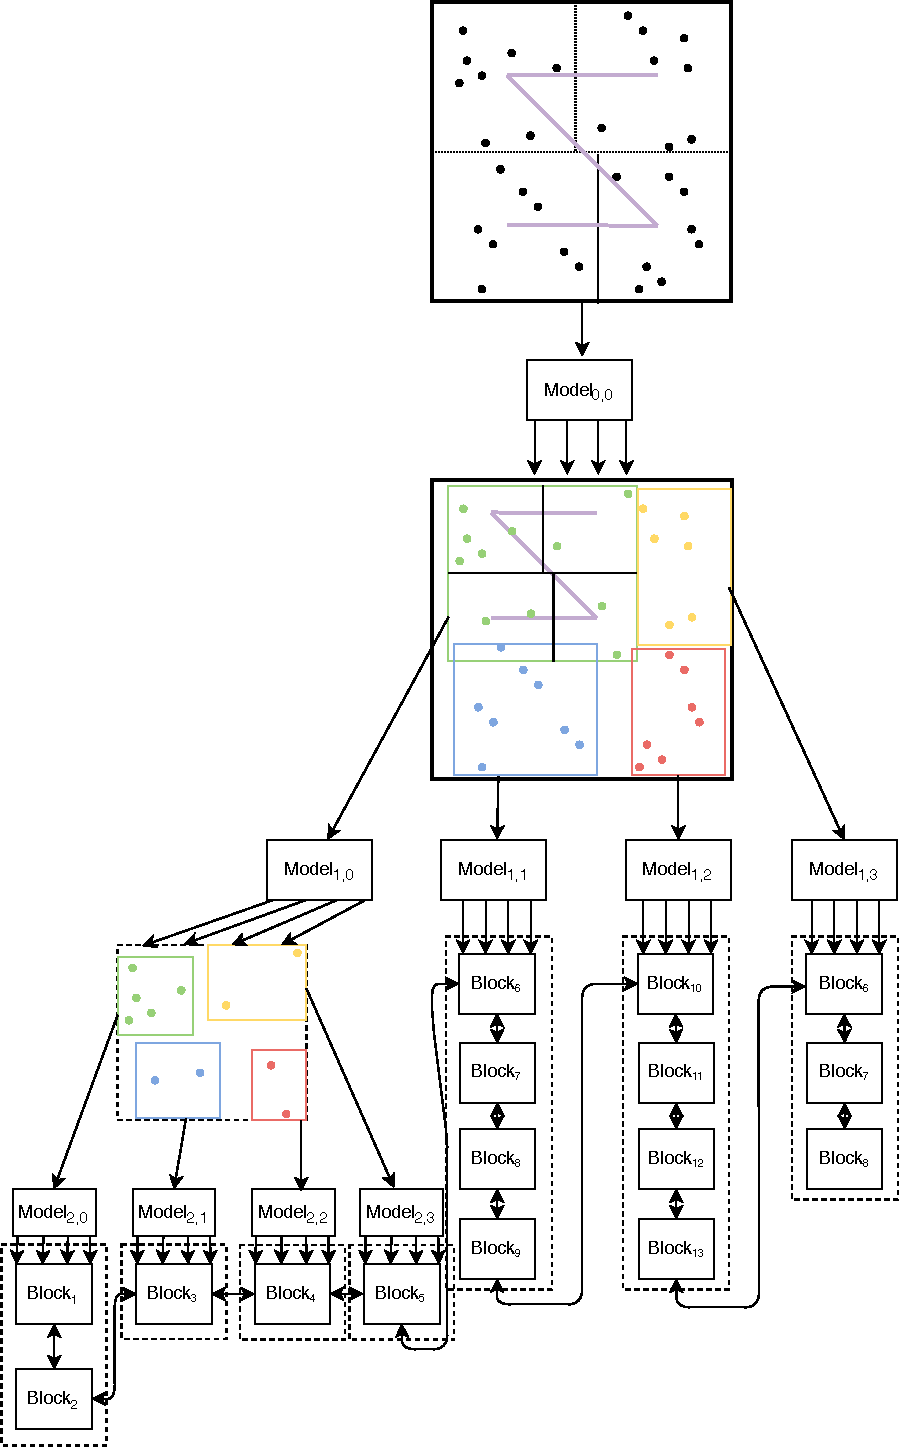
\includegraphics[scale=0.7]{Figures/rsmi.pdf}
\caption{RSMI}
\label{fig:rsmi}
\end{figure}

The recursive spatial model index (RSMI) \cite{Qi:2020uz} is another spatial data index that incorporates the Z-order curve and the RMI. Data points in the spatial space are first mapped to a $n \times n$ grid to describe the rank space. Then a Z-order curve maps every point on the rank space with a curve value. All points are sorted in ascending order based on the curve value, then points can be packed into a block by $p.blk = [p.rank \cdot n/B]$, where B is the capacity of a block. Then, a regression model is trained to predict the $p.blk$ for given point coordinate. 

For a larger scale data set, the RSMI partition all data points into a certain size of the grid. Each of the grid cells contains up to a certain number of data points. At the top level, the model is predicting a value that is not directly the exact matching result. Then, we can regroup points with the same block curve value. The partition will be repeated to follow in the same manner, the learned model in each partition predicts which sub-partition the point belongs to. Once the partition is completed, data points along with block id from preceding and subsequent blocks are stored in each block. The pointer of block id makes it easier for access and searching in blocks at a different level. 

To execute a point query in RSMI, the coordinates of the searching point is used as the input query that can be fed into the learned model. The searching process is done recursively, starting from the root model, the prediction value is pointing to the submodel at the next level. The searching procedure is repeated recursively until reaching the leaf model. The output prediction value from the leaf model is the block ID of the input point. At the final stage, we can examine the block and its neighbouring block within an error bound. 

For the range query, we can locate the minimum and maximum curve value $q_min$ and $q_max$ from the input query. Then it retrieves all the candidate points between $q_min$ and $q_max$. Finally, candidate points can be filtered out from the window range, and remaining points will be the result. 

The K nearest neighbour query in RSMI starts with searching in a small region around the input query key. It will keep searching in the expanding region until $k$ points are found. A window query will be performed when the search region is expanding. Measuring the distance from the point to the query point, and comparing to the existing points that have the minimum distance in the result. The initial search region size can be determined by the number of points and number of regions for the uniformly distributed data. Two skew parameters are introduced to adjust the search region based on the skewness of the data. 

The result shows that the RSMI has a good performance on the point query, the number of block accesses is significantly lower than traditional data indexes and the ZM model. A disadvantage of the RSMI is that the training time cost is much higher compared to the traditional methods. The training time of RSMI is also higher than the ZM model since sorting is needed for each partition.




\subsection{Flood}

\begin{figure}[ht]
\centering
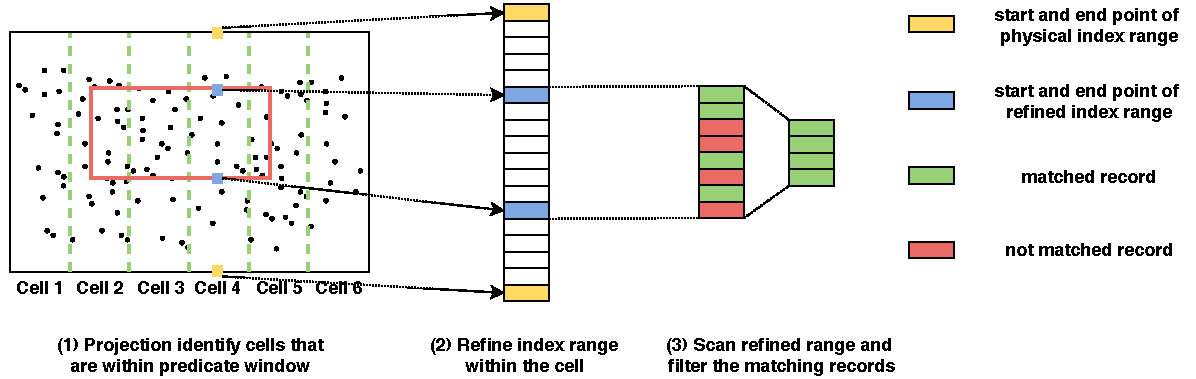
\includegraphics[width=\textwidth]{Figures/flood.pdf}
\caption{Flood}
\label{fig:flood}
\end{figure}

Flood \cite{Nathan:2019wc} claims to be the first learned multi-dimensional in-memory index, which is based on the point access method grid file. The Flood model first to preprocess offline to choose an optimal layout for indexing, then an online component to handle executing queries. 

The model breaks down into three parts: Projection, Refinement and Scan. Similar to the traditional grid file, projection first to match a query is to locate the cell containing the search point, which is to identify the range of position in storage. Compared to z-address, points in the columns that are along x and then sorted by their y-values, creating the serialization order. Then, refinement can narrow down the range of search. When query overflows the sort dimension, Flood can take advantage of the ordering of points within each cell to further refine the physical index ranges. The final step is to scan and find the matched query filter. The model time complexity depends on the weight for each step $w_s$, $w_r$ and $w_s$ and size of cells and scanning points. 

Flood also uses a piecewise linear model(PLM) to train the CDF. By using PLM, the partition boundary between each column is not equally spaced. A flattened layout, as referred in the paper, is introduced to correlate with unevenly distributed data. They also mentioned that modelling based on a single-dimensional attribute was sufficient to reach an equal number of points in each partition. 

Compared to other traditional multidimensional data structures, Flood shows significant performance improvement on query time. In measuring varying query selectivity, Flood also works well and outperforms other traditional methods. 


\subsection{Tsunami}
A more recent study from the same authors of the Flood model proposed an improvement index Tsunami \cite{Ding:2020we} based on the Flood model. Flood has some limitations when training on the non-uniform data distribution, each grid cell can have uneven distribution of data points. To address this problem, Tsunami proposes a data structure composed of the Grid Tree and Augmented Grid. 

The Grid Tree divides space into partitions based on the values of split dimension. Each partition contains a number of data points, which are stored in the internal node of the Gird Tree. An optimization is applied to the Grid Tree to minimize the query skew, by setting the split value that reduces the skew the most. 

The Augmented Grid can correlate the points within each sub-region. Several different strategies can be applied to create partitions. Notably, the strategy used in Flood is $CDF$ on $X$ independently from other dimensions. It can use a conditional $CDF(X|Y)$ that X dependent on another dimension $Y$. It can also use a functional mapping to some dimension other than $X$. They used adaptive gradient descent to optimize the augmented grid for the lowest average predicted query time and search space size. 

The performance result shows that query time for Tsunami is 6$\times$ faster than Flood and 11$\times$ faster than the traditional index. The index size of the Tsunami is also much less than other indexes. The advantage of Tsunami is that it proposed strategies for data correlation to produce a more uniformly distributed data from a skewed dataset. There is still room for improvements, as mentioned in the paper, functional mapping can not handle outliers very well, the error bound can be enlarged; and the Augmented Grid can not handle higher dimensional data. 

\subsection{qd-tree}
Qd-tree \cite{Yang:2020ev} is a high-dimensional data space partitioning binary tree, which is similar to the k-d tree. The qd-tree approaches the query task from a deep reinforcement learning-based framework. The structure of the qd-tree is built upon the binary tree. Each node in the tree contains data records that belong to the multidimensional data. The root node of the tree holds all the information for the entire dataset. 

The strategy of querying entry in the tree is using a concept of routing data. Data is stored in the blocks on storage. Every record starts routing at the root of the tree, the same as most of the hierarchical structure, the record will recursively traverse down the tree. At each node, the tagged predicate $p$ is evaluated on the record. Each predicate in the node does range comparison ($\{<, \leq, >, \geq\}$) and equality comparison ($=$). A record at the node does a series of range comparisons to decide which leaf (left or right) to go.  Eventually, the record will be landed in the leaf node. The leaf node represents the physical location of the record on the disk. The block ID (\texttt{BID}) is stored along with the record on the leaf, indicating where the record belongs to. 

The Greedy approach is beginning with a single root node that contains all the nodes. Then iterate through all the nodes to split the leaf node that is larger than $2b$ into two children nodes, the size of each of the children nodes is at least $b$. The Greedy approach has been reported \cite{Yang:2020ev} to work well to reach the local optimum and may be global suboptimality. 

The Deep RL method is a black box learning process without assumption on the data distribution or query. The Deep RL agent Woodblock is built on top of the Markov Decision Process (MDP). It defines the state space to be any subspace of entire data space, and action space to be the set of splits. The Woodblock agent contains two parameterized networks: 
\begin{enumerate*}
    \item \textit{Policy Network}, which takes a state and emits a probability distribution over an action space.
    \item \textit{Value Network}, which estimates an expected cumulative reward for a given state.
\end{enumerate*}
The learning process trained through a series of episodes: 
\begin{enumerate}
    \item Starts from a node off from the queue,
    \item Evaluates the policy at current state,
    \item Choice an action from the output distribution,
    \item Applies this action on the current node to produce a new node.
\end{enumerate}

A stopping condition is necessary for ending the episode training. As it is defined in the tree structure that the leaf node must contain at least $b$ records, the agent will continue to make cuts on the current node if it contains more than $b$ records. Overlapping region existing in the qd-tree. To handle such data redundancy in the leaf node, qd-tree proposed a relaxed cutting condition that allows one of the children nodes to have a size smaller than $b$.  


\subsection{LISA}
LISA proposed by Li \cite{Li:2020ki}, designated to generate data layout that allows using machine learning models to search in an arbitrary spatial dataset that is stored in the disk pages. Similar to many popular traditional approaches, LISA partitioning space into a series of grid cells, and numbering the cells along a sequence of axes. It builds a learned regression model $SP$ to map the keys distribution into different shards, and assign an id for each shard. All shards preserve order concerning the corresponding interval in the mapped data. Keys in shards are stored in several disk pages, which means that one shard might contain keys from different pages. At the final stage, local models are required for page address lookup for the given query. 

LISA also adopted a piecewise linear function as the shard prediction function. The piecewise linear function is a monotonic regression model, and it allows the mapped values to be sorted. Therefore, the operations for searching members of different partitions at the bottom level is efficient. The range query in LISA access to the keys that belong to the search region. Similar to traditional spatial indexes that applied \textbf{overlapping regions} technique, since the space partition might divide keys from different disk pages, it has to scan the overlapped pages in local models. For a KNN query, the given point and the number of return values k, LISA will estimate the distance bound base on the query. Then, the keys remaining within the bound are selected to perform repetitive range queries, until we get K nearest keys. 

Compared to traditional such as R-Tree, KD-Tree, the advantage of LISA is that it benefits from the learned monotonic function. The learned monotonic function allows the mapping order of keys to be sorted, keys that to be appended to the structure are naturally sorted. Hence key lookup in neighbouring value and update handling in LISA is easy. Even though it still has overlapping regions in the local models, LISA still does less data updating than R-Tree. 

\subsection{ML-Index}
The ML-Index \cite{Davitkova:2020dx} is another learned index for multidimensional data, and it supports point query, range query and KNN query. The ML-Index consists of two main components, the first part of the structure is to convert and scale the two-dimensional data into one dimension, and the second part is to use an RMI model as mentioned above by Kraska to learn the CDF of the data distribution. 

The upper part of the algorithm is to scale a group of points that are similar to each other, and project into one-dimension. The first scaling method is to map distances of all points to a single reference point and use the distances as keys. It works for small datasets, but it is hard to scale to larger datasets. The second scaling method is called iDistance by Jagadish et al. \cite{jagadish2005idistance}, $key = i \times c + dist(O_i, d_l)$, where $i$ is the index of the closest reference point $O_i$, and a constant $c$ partitions the points into predefined ranges and stretches the range according to its value. The third method calculates the offset value as the scaling value $key = \text{offset}_i + dist(O_i, d_L)$, where the offset is calculated by sum of the radii of every partition that is based on their arbitrary reference points.  

The second part of the index is to build a recursive learned index as described in Kraska's paper. Instead of building multiple stages models in the original paper, the ML-Index uses only two stages to reduce expected error by increasing the number of models in the second stage. 

The point query procedure is the same as RMI, which uses scaled values to predict bounds containing the expected query result from $[pos - err, pos + err]$. The range query iterates through the reference points and calculates the closest and furthest point for each reference point from the query range. Then issue the model prediction to find keys that are within the range. For the KNN query, the algorithm first predicts the position of the query key to locating the starting point of the search. 


\subsection{PolyFit}
PolyFit \cite{li2020polyfit} uses piecewise polynomial functions to process approximate range aggregate queries. Aggregate functions including COUNT, SUM, MIN and MAX. The key cumulative functions are extracted from those aggregate functions. Then the measured key cumulative function is used to construct the index. 

The PolyFit index is built upon polynomial fitting for an interval of data. The polynomial function can achieve a better approximation of data distribution when compared to linear regression or piecewise linear regression. It is hard to fit the whole dataset with one polynomial function. Therefore, it also utilizes multiple polynomial functions to reduce the fitting error, which could get the approximate function more accurately. Memory consumption is also worth considering, one way is to use dynamic programming to minimize the number of polynomial functions while fitting the dataset well. Authors proposed Greedy Segmentation method (GS), it inserts one more key into the interval incrementally, then checks whether the interval can fulfill the bounded error constraint. 

The PolyFit can be extended for two-dimensional queries. Similar to the one dimensional range aggregate queries, it estimates the key cumulative function with two keys for COUNT query. Then follow the same idea from GS to utilize the number of polynomial functions. However, the GS method takes $O(n^2)$ to obtain the minimum number of segmentations. They use a Quad-tree based method to get the segmentations. If a segmentation does not fulfill the error guarantee, the space partition can be continuously broken into four smaller partitions. 



\section{Research Gaps}
Researchers have different perspectives on constructing access methods for multidimensional data, from a traditional hierarchical structure to a learned index. 

The learned index is opening a new page for traditional data access methods by applying machine learning. The optimization of the machine-learned model seems to have a big advantage over traditional hierarchical methods. The complexity of the model is scaled by the width $h$ of the model and input length $N$: $O(hN)$. The linear model only using multiplication and addition operation: $w*x+b$, to calculate the prediction value. As a result, the Learned Index does not have searching phrases between stages. Consequently, it can achieve constant searching time complexity, while hierarchical structure B-Tree requires $O(logn)$ searching time. On space complexity, the learned index also has an advantage over B-Tree. For inserting a new key, we might not need to re-train the entire model depending on the key. The new key could fall into a range at the next stage, the root stage model can predicate the same pointer to the next model that has the same range of keys. 

However, there are some drawbacks to the learned index. For indexing, finding the min and max error of a position is more interesting to us. A typical machine learning model is to generalize the result, make it more suitable for real-world data. In the learned index, we wish to minimize the error as close to 0 as possible to achieve accurate results. It is different from a data science aspect problem, the fitting curve is preferred to overfit the dataset instead of generalizing the model. 

The neural net model at the top stage does not produce the exact position of the key, requiring a 'last-mile' searching phase. The accuracy problem still exists in the ‘last-mile’ phase, which means the model still relies on hierarchical structure and traditional indexing method. The B-Tree is cache efficient. Machine learned models require all weights to compute a prediction, in which the multiplication and addition cost more memory. 
 

Both Wang \cite{Wang:2019ks} and Nathan \cite{Nathan:2019wc} represent multidimensional spatial data in a linear vector space. One of the difficulties of spatial data is the consistency of simultaneity ordered on different dimensions. For example, on a 2D spatial data, the growth of the Y-axis does not grow simultaneously along the X-axis. 


The learned ZM index is trying to solve multidimensional problems in a one-dimensional way. The z-order curve or z-address is aiming to solve the consistency of simultaneously ordered spatial data on different dimensions. Interleaving bits of two-point value in a coordinate can convert the multidimensional data into one dimension. Applying the learned index model from Kafle \cite{Kafle:2017dy}, we could achieve a similar result as the learned B-Tree model. 

The advantage\cite{Ding:2020we} of the Flood is that the query performance can be boosted by automatically adjusting the number of partitions in each dimension. The more partitions in the data space, the fewer points are needed to be scanned. A drawback of Flood is that it is not optimized for skewed data. For a query that is non-uniform, it will scan a large range of points until reaching the result. 


\begin{adjustbox}{width={\textwidth}, totalheight={\textheight},keepaspectratio}%
\footnotesize
\newcommand*\rot[1]{\hss\rotatebox[origin=br]{-60}{#1}}
\newcommand*\rotNarrow[1]{\hbox to2em{\hss\rotatebox[origin=br]{-60}{#1}}}
\newcommand*\feature[1]{\ifcase#1 -\or\LEFTcircle\or\CIRCLE\fi}
\newcommand*\f[5]{\feature#1&\feature#2&\feature#3&\feature#4&\feature#5}
\newcommand*\ff[6]{\feature#1&\feature#2&\feature#3&\feature#4&\feature#5&\feature#6}
\newcommand*\fff[8]{\feature#1&\feature#2&\feature#3&\feature#4&\feature#5&\feature#6&\feature#7&\feature#8}
\newcommand*\ex[4]{#1&\ff#2&\f#3&\fff#4}

\begin{threeparttable}
\caption{Comparison of Data Indexes}
\label{tab:features}

\begin{tabular}{@{}l c@{}c@{}c@{}c@{}c@{}c@{} | c@{}c@{}c@{}c@{}c |  c@{}c@{}c@{}c@{}c@{}c@{}c@{}c}
\toprule
    Index Type
    & \multicolumn{6}{c}{Traditional Spatial Indexes}
    & \multicolumn{5}{c}{Learned Indexes} 
    & \multicolumn{8}{c}{Learned Spatial Indexes}\\
\midrule
% rotated items
 Model Name
 & \rot{Grid File}
 & \rot{MOLHPE}
 & \rot{K-D-Tree}
 & \rot{BSP-tree}
 & \rot{Quadtree}
 & \rot{R-Tree}
 %
 & \rot{RMI}
 & \rot{ALEX}
 & \rot{PGM-index}
 & \rot{RadixSpline}
 & \rot{FITing-Tree}
%  & \rotNarrow{PolyFit}
 
 %
 & \rot{ZM}
 & \rot{RSMI}
 & \rot{Flood}
 & \rot{Tsunami}
 & \rot{qd-tree}
 & \rot{LISA}
 & \rot{ML-Index}
 & \rot{PolyFit}\\

\midrule
\ex{Top-down Construction} {222220}{22000}{22220222} \\
\ex{Bottom-up Construction} {000002}{00222}{00002000} \\
\ex{Single-pass Training} {222221}{00222}{00000000} \\
\ex{Linear Structure} {020000}{00010}{00000000} \\
\ex{Hierarchical Structure} {002222}{22202}{22002022} \\
\ex{Grid Layout} {200000}{00000}{00220201} \\

\midrule
\ex{CDF approximation} {000000}{22222}{22222222} \\
\ex{Piecewise Linear Model} {000000}{00202}{00200200} \\
\ex{Recursive Model} {000000}{22202}{22000022} \\
\ex{Reinforcement Learning} {000000}{00000}{00002000} \\
\ex{Require Sorted Data} {000000}{22221}{21002222} \\
\ex{Require Local Search} {200000}{10002}{22222222} \\
 
\midrule
\ex{Transformation} {010000}{00000}{22000000} \\
\ex{Overlapping Regions} {000002}{22200}{02000020} \\
\ex{Clipping} {002000}{00000}{00000000} \\
\ex{Multiple Layers} {100000}{00000}{00000000} \\
\ex{Space Partitioning} {100000}{00000}{00220202} \\

\midrule
\ex{Point Query} {222222}{22222}{22222222} \\
\ex{Range Query} {222222}{20002}{22001222} \\
\ex{Nearest Neighbour Query} {202222}{00000}{02000220} \\

\bottomrule
\end{tabular}

\begin{tablenotes}
\item \hfil$\feature2=\text{provides features}$; 
$\feature1=\text{partially provides features}$;
$\text{\feature0}=\text{does not provide features}$;
% \item \hfil\textsuperscript{\dag}has academic publication;
% \textsuperscript{*}end-user tool available
\end{tablenotes}

\end{threeparttable}

% \end{table}
\end{adjustbox}



\section{Summary}
From this review, we have perceived the background knowledge and design flows of some popular traditional spatial indexes, the learned index for one-dimensional data and current state-of-art learned spatial indexes. There are no perfect index methods, each method has its strengths and weaknesses. 

To design a learned spatial index, we might consider some recipes from the current learned models and spatial indexes. The learned CDF curve can map an approximate shape of data distribution. Finding a fuzzy position of key only costs a complexity of prediction depending on the model. Transformation techniques in the spatial index provide a way to convert multidimensional spatial objects into one-dimensional data. Both ZM and RSMI applied Z-order space-filling curves in their models, so we can store spatial data in one-dimensional index fashion. Overlapping regions can handle complex operations for spatial queries, but overlapping areas can lead to searching on redundant paths in a hierarchical structure like R-Tree and even in the RMI. 

Most learned indexes are trying to optimize between space and time. The RMI looks for the position key regarding an upper bound and a lower bound. This bounded range can be large if the model under-fits the data. However, to train a well-fitted model, it requires more training time and more complex models. A complex model can be more expensive when inference during searching.  The PGM-index offers a flexible turning strategy for either optimizing space for a query time constraint or optimizing query time for a space constraint. It is done by controlling the number of segments in the model. Radix spline’s approach to this problem is to build a separate Radix table to look up a range of query points. The size of the Radix table can grow larger with the increase of query precision. 

Integrating the learned model with traditional spatial indexes achieved good performance. The Flood follows the idea from the Grid File, it partitions the data layout into numbers of Grid cells, then narrows down the search region. The Flood learns from the data distribution and builds the model to determine the location of query points. The Tsunami further improves the skewed data handling in Flood by using functional mapping and conditional CDFs. 
